\section{A range space of shortest paths}\label{sec:centrsamplrangeset}
We now define a range space of the shortest paths of a graph $G=(V,E)$, and present 
a strict upper bound to its VC-dimension. %We show that this upper bound is strict. 
We use the range space and the bound in the analysis of our algorithms for estimating
the betweenness centrality of vertices of $G$.

The domain of the range space is the set $\mathbb{S}_G$ of all shortest
paths between vertices of $G$. The set $\range_G$ of ranges contains a subset of
$\mathbb{S}_G$ for each vertex $v\in V$, that is the set $\mathcal{T}_v$ of
shortest paths that $v$ is internal to:
\[
\range_G = \{\mathcal{T}_v ~:~ v\in V\}\enspace.
\]
We denote this range space as $\range_G$.

\begin{lemma}\label{lem:vcdimuppbound}
  %Given a graph $G=(V,E)$ with vertex-diameter $\Delta_G$, the range space
  %$\range_G$ associated to the shortest paths in $G$ has VC-dimension
  $\VC\left((\mathbb{S}_G,\range_G)\right)\le\lfloor\log_2(\VD(G)-2)\rfloor+1$.
\end{lemma}

\begin{proof}
Let $\ell>\lfloor\log_2(\VD(G)-2)\rfloor+1$ and assume for the sake of contradiction
that $\VC\left((\mathbb{S}_G,\range_G)\right)=\ell$. From the definition of the VC-dimension there is a set
$Q\subseteq\mathbb{S}_G$ of size $\ell$ that is shattered by $\range_G$. Let $p$ be
an element of $Q$. There are  $2^{\ell-1}$ non-empty subsets of
$Q$ containing the path $p$. Let us label these non-empty subsets of $Q$ containing $p$ as
$S_1,\dotsc,S_{2^{\ell-1}}$, where the labelling is arbitrary.
Given that $Q$ is shattered, for each set $S_i$ there must be a range $R_i$ in
$\range_G$ such that $S_i=Q\cap R_i$. Since all the $S_i$'s are
different from each other, then all the $R_i$'s must be different from each
other. Given that $p$ belongs to each $S_i$, then $p$ must also belong to each
$R_i$, that is, there are $2^{\ell-1}$ distinct ranges in $\range_G$ containing
$p$. But $p$ belongs only to the ranges corresponding to internal vertices of
$p$, i.e., to vertices in $\mathsf{Int}(p)$. This means that the number of ranges
in $\range_G$ that $p$ belongs to is equal to $|p|-2$. But $|p|\le\VD(G)$, by
definition of $\VD(G)$, so $p$
can belong to at most $\VD(G)-2$ ranges from $\range_G$. Given that
$2^{\ell-1}>\VD(G)-2$, we reached a contradiction and there cannot be $2^{\ell-1}$
distinct ranges containing $p$, hence not all the sets $S_i$ can be expressed as
$Q\cap R_i$ for some $R_i\in\range_G$. Then $Q$ cannot be shattered and
$\VC\left((\mathbb{S}_G,\range_G\right))\le\lfloor\log_2(\VD(G)-2)\rfloor+1$.%\qed
\end{proof}

\paragraph{Unique shortest paths}\label{sec:centrsamplrangeunique}
In the restricted case when the graph is undirected and
every pair of distinct vertices has either none or a unique shortest path
between them, the VC-dimension of $(\mathbb{S}_G,\range_G)$ reduces %collapses 
to a \emph{constant}. This is a somewhat surprising result with interesting
consequences. From a theoretical point of view, it suggests that there should be
other characteristic quantities of the graph different from the vertex diameter
that control the VC-dimension of the range space of shortest paths, and these
quantities are constant on graph with unique shortest paths between vertices.
From a more practical point of view, we will see in
Sect.~\ref{sec:centrsamplalgo} that this result has an impact on the sample size
needed to approximate the betweenness centrality of networks where the
unique-shortest-path property is satisfied or even enforced, like road
networks~\citep{GeisbergerSS08}. In particular, the resulting sample size will
be \emph{completely independent} from any characteristic of the network, and
will only be a function of the parameters controlling the desired approximation
guarantees. 

\begin{lemma}\label{lem:vcdimuppboundunique}
  Let $G=(V,E)$ be an undirected graph with $|\mathcal{S}_{uv}|\le1$ for all
  pairs $(u,v)\in V\times V$. Then $\VC\left((\mathbb{S}_G,\range_G)\right)\le 3$.
\end{lemma}

\begin{proof}
  First of all, notice that in this restricted setting, if two different
  shortest paths $p_1$ and $p_2$ meet at a vertex $u$, then they either go on
  together or %at a certain point 
  they separate never to meet again at any other
  vertex $v\neq u$. This is easy to see: if they could separate at $u$ and then
  meet again at some $v$, then there would be two distinct shortest paths
  between $u$ and $v$, which is a contradiction of the hypothesis. Let us denote
  this fact as $\mathsf{F}$.

  Assume now that $\VC\left((\mathbb{S}_G,\range_G)\right)>3$, then there must be a set
  $Q=\{p_1,p_2,p_3,p_4\}$ of four shortest paths that can be shattered by
  $\range_G$. Then there is a vertex $w$ such that $\mathcal{T}_w\cap Q=Q$, i.e.,
  all paths in $Q$ go through $w$. Let $x$ be the farthest predecessor of $w$
  along $p_1$ that $p_1$ shares with some other path from $Q$, and let $y$ be
  the farthest successor of $w$ along $p_1$ that $p_1$ shares with some other
  path from $Q$. It is easy to see that if either $x$ or $y$ (or both) do not
  exist, then $Q$ cannot be shattered, as we would incur in a contradiction of
  fact $\mathsf{F}$. 
  
  Let us then assume that both $x$ and $y$ exist.
  Let $Q_x=\mathcal{T}_x\cap Q$ and $Q_y=\mathcal{T}_y\cap Q$.
  Because of fact $\mathsf{F}$, all paths in $Q_x$ must go through the same vertices
  between $x$ and $w$ and all paths in $Q_y$ must go through the same vertices
  between $w$ and $y$. This also means that all paths in $Q_x\cap Q_y$ must go
  through the same vertices between $x$ and $y$. If $Q_x\cup Q_y\neq Q$, let
  $p^*\in Q\setminus(Q_x\cup Q_y)$. Then from the definition of $x$ and $y$ and
  from fact $\mathsf{F}$ we have that there is no vertex $v$ such that
  $\mathcal{T}_v\cap Q=\{p_1,p^*\}$, which implies that $Q$ can not be
  shattered. 
  
  Suppose from now on that $Q_x\cup Q_y=Q$.  If $Q_x\cap Q_y=Q$, then
  all the paths in $Q$ go through the same vertices between $x$ and $y$. From
  this and the definition of $x$ and $y$ we have that there is no vertex $v$
  such that, for example, $\mathcal{T}_v\cap Q=\{p_1,p_2\}$, hence $Q$ cannot be
  shattered. Suppose instead that $Q_x\cap Q_y\neq Q$ and let $S=(Q_x\cap
  Q_y)\setminus\{p_1\}$. If $S\neq\emptyset$ then there is at least a path
  $p'\in S$ which, from the definition of $S$ and fact $\mathsf{F}$, must go
  through all the same vertices as $p_1$ between $x$ and $y$. Moreover, given
  that $Q_x\cap Q_y\neq Q$, there must be a path $p^*\in Q\setminus\{p_1\}$
  different from $p_1$ such that $p^*\notin S$. Then, from the definition of
  $x$, $y$, and $S$, and from the existence of $p'$, there can be no vertex $v$
  such that $\mathcal{T}_v\cap Q=\{p_1,p^*\}$, hence $Q$ cannot be shattered.
  Assume now that $S=\emptyset$ and consider the case $Q_x=\{p_1,p_2,p_3\}$,
  $Q_y=\{p_1,p_4\}$ (all other cases follow by symmetry with this case).
  Consider the set $\{p_1,p_3\}$. From the definition of $x$ and $Q_x$, and from
  fact $\mathsf{F}$ we have that there can not be a vertex $v$ between the end
  point of $p_1$ before $x$ and $w$ such that $\mathcal{T}_v\cap Q=\{p_1,p_3\}$.
  At the same time, from the definition of $y$ and from fact $\mathsf{F}$, we
  have that such a $v$ can not be between $w$ and the end point of $p_1$ after
  $y$. This implies that $Q$ can not be shattered.

  We showed that in all possible cases we reached a contradiction and $Q$,
  which has size $4$, can not be shattered by $\range_G$. Hence
  $\VC\left((\mathbb{S}_G,\range_G)\right)\le 3$.
\end{proof}

It is natural to ask whether the above lemma or a similar result also holds for
\emph{directed} graphs. Fact $\mathsf{F}$ does not hold for directed graphs so
the above proof does not extend immediately. In Fig.~\ref{fig:counterexample} we show
a directed graph. For any pair of vertices in the graph, there is at most a
unique shortest path connecting them. Consider now the
following four directed shortest paths:
\begin{itemize}
  \item $p_A=\{1,2,4,6,7,12,13,14,16,17,18,22,21\}$
  \item $p_B=\{8,9,10,5,12,13,14,16,17,18,23,26,27\}$
  \item $p_C=\{25,24,26,18,19,15,14,7,6,5,4,3\}$
  \item $p_D=\{23,20,22,17,16,15,14,7,6,5,10,11\}$
\end{itemize}
It is easy to check that the set $\{p_A,p_B,p_C,p_D\}$ is shattered, so the
above lemma is not true for directed graphs. It is an open problem whether it is
true for a different constant.

\begin{figure}
\centering
\begin{tikzpicture}
\GraphInit[vstyle=Normal]
\SetUpEdge[style={->}]
\Vertex{1}
\WE(1){2}
\SO(2){4}
\EA(4){3}
\SO(4){5}
\WE(5){10}
\NO(10){9}
\NO(9){8}
\SO(10){11}
\SO(4){5}
\EA(5){6}
\SO(6){12}
\EA(6){7}
\SO(7){13}
\EA(7){14}
\EA(14){16}
\SO(16){15}
\EA(16){17}
\EA(17){18}
\SO(17){19}
\EA(18){26}
\NO(18){22}
\WE(22){21}
\NO(22){20}
\WE(20){23}
\SO(26){27}
\NO(26){24}
\NO(24){25}
\Edge(1)(2)
\Edge(2)(4)
\Edge(4)(3)
\Edge(8)(9)
\Edge(9)(10)
\Edge(10)(11)
\Edge(5)(4)
\Edge[style={->,bend left}](5)(10)
\Edge[style={->,bend left}](10)(5)
\Edge(5)(12)
\Edge(12)(13)
\Edge(4)(6)
\Edge(6)(5)
\Edge[style={->,bend left}](6)(7)
\Edge[style={->,bend left}](7)(6)
\Edge(7)(13)
\Edge(13)(14)
\Edge(14)(7)
\Edge(15)(14)
\Edge(14)(16)
\Edge(16)(15)
\Edge[style={->,bend left}](16)(17)
\Edge[style={->,bend left}](17)(16)
\Edge(18)(19)
\Edge(19)(15)
\Edge(17)(18)
\Edge(18)(22)
\Edge(22)(17)
\Edge(22)(21)
\Edge(20)(22)
\Edge(23)(20)
\Edge[style={->,bend left}](18)(26)
\Edge[style={->,bend left}](26)(18)
\Edge(26)(27)
\Edge(24)(26)
\Edge(25)(24)
\end{tikzpicture}
\caption{Directed graph $G=(V,E)$ with $|\mathcal{S}_{uv}|\le1$ for all pairs
$(u,v)\in V\times V$ and such that it is possible to shatter a set of four
paths.}
\label{fig:counterexample}
\end{figure}


\subsection{Tightness}\label{sec:centrsampltightness}
The bound presented in Lemma~\ref{lem:vcdimuppbound} is strict in the sense that
for each $d\ge 1$ we can build a graph $G_d$ with vertex-diameter
$\VD(G_d)=2^d+1$ and such that the range space $(\mathbb{S}_{G_d},\range_{G_d})$ associated to the set of
shortest paths of $G_d$ has VC-dimension exactly
$d=\lfloor\log_2(\VD(G_d)-2)\rfloor+1$. 
%For the sake of clarity, we will discuss
%only the case of undirected graphs with equal edge weights, but all we say can
%be easily adapted to the general case.

We now introduce a class $\mathcal{G}=(G_d)_{d\ge 1}$ of graphs indexed by $d$.
The graphs in $\mathcal{G}$ are the ones for which we can show the tightness of
the bound to the VC-dimension of the associated range space.
We call the graph $G_d\in\mathcal{G}$ the \emph{$d$\textsuperscript{th} concertina graph}.
Figure~\ref{fig:centrsampltightgraphs} shows $G_1$, $G_2$, $G_3$, and $G_4$. The
generalization to higher values of $d$ is be straightforward.
By construction, $\VD(G_d)=2^d+1$, so that
$\lfloor\log_2(\VD(G_d)-2)\rfloor+1=d$. The $3(2^{d-1})$ vertices of $G_d$ can
be partitioned into three classes, \emph{top}, \emph{bottom}, and \emph{middle},
according to their location in a drawing of the graph similar to those in
Fig.~\ref{fig:centrsampltightgraphs}. $G_d$ has $2^{d-1}-1$ top vertices, $2^{d-1}-1$ bottom vertices, and
$2^{d-1}+2$ middle vertices. For each top vertex $v$, let $\mathsf{f}(v)$ be the
\emph{corresponding bottom vertex}, i.e., the bottom vertex $u$ whose neighbors
are the same middle vertices that are neighbors of $v$. Among the middle
vertices, the two with degree 1 are special and are called the \emph{end
vertices} of $G_d$ and denoted as $v_\ell$ and $v_\mathrm{r}$, where the
labels can be arbitrarily assigned. We now build a set $Q$ of $d$
shortest paths from $v_\ell$ to $v_\mathrm{r}$ and show that it is
shattered by $\range_{G_d}$, therefore proving that
$\VC\left((\mathbb{S}_{G_d},R_{G_d})\right)\ge d$.
This fact, together with Lemma~\ref{lem:vcdimuppbound}, allows us to conclude
that $\VC\left(\mathbb{S}_{G_d},R_{G_d})\right)=d$. 

\begin{figure}[htbp]
  \centering
  \subcaptionbox{Examples of concertina graphs $G_d$ for
  $d=1,2,3,4$.\label{fig:centrsampltightgraphs}}{
    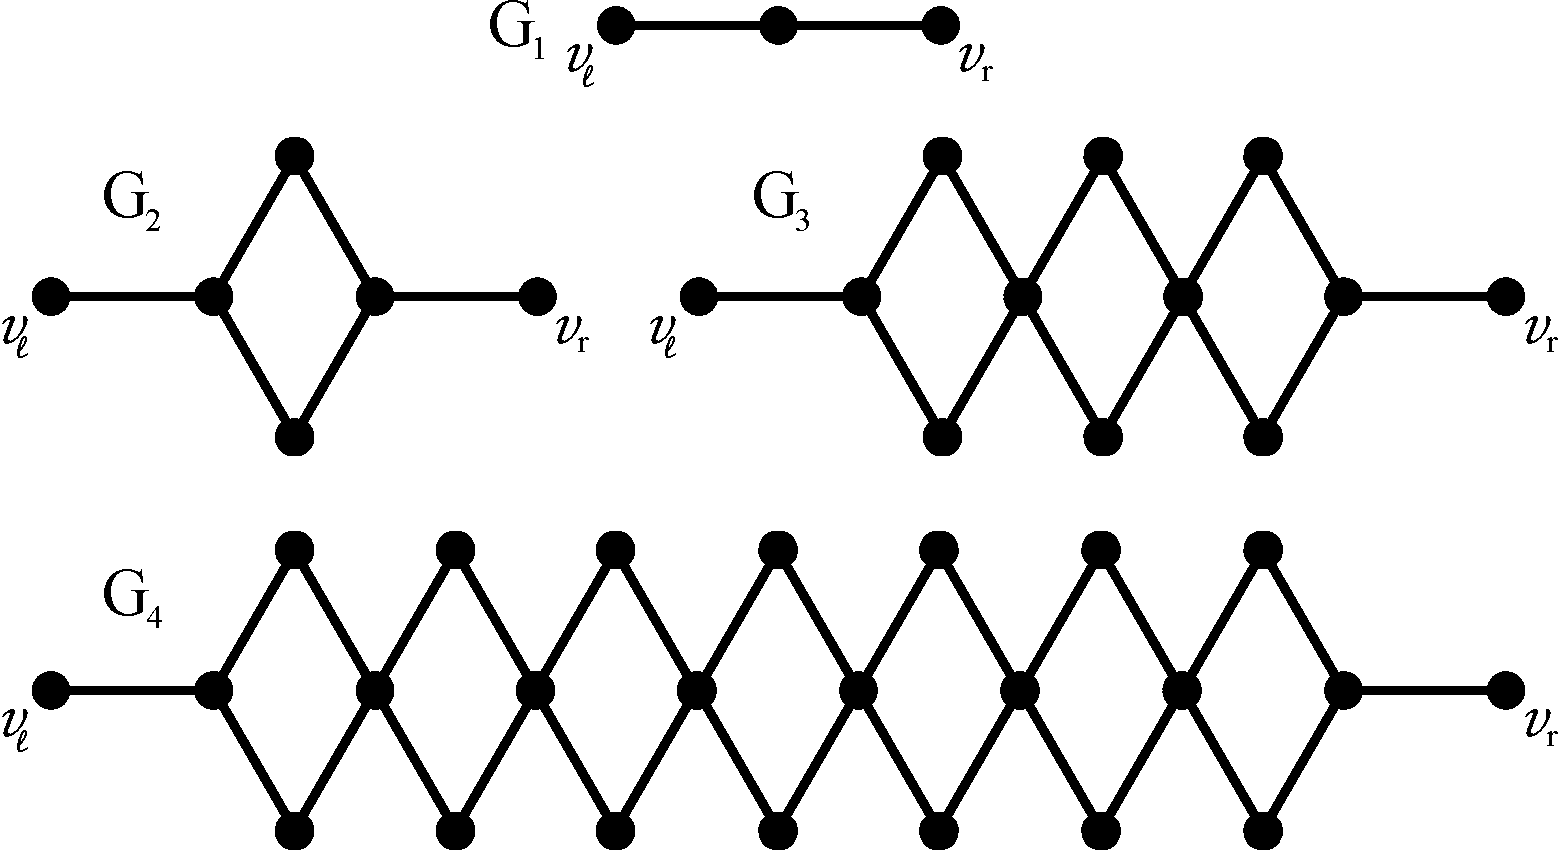
\includegraphics[width=0.3\textwidth,keepaspectratio]{centrsampl/figures/eps/tight}
    }
  \hfill
  \subcaptionbox{An example of the $\mathsf{r}$ map for $G_3$. The set next to
  each top and bottom vertex $u$ is the set $s$ such that
  $\mathsf{r}(s)=u$.\label{fig:centrsamplmapexample}}{
    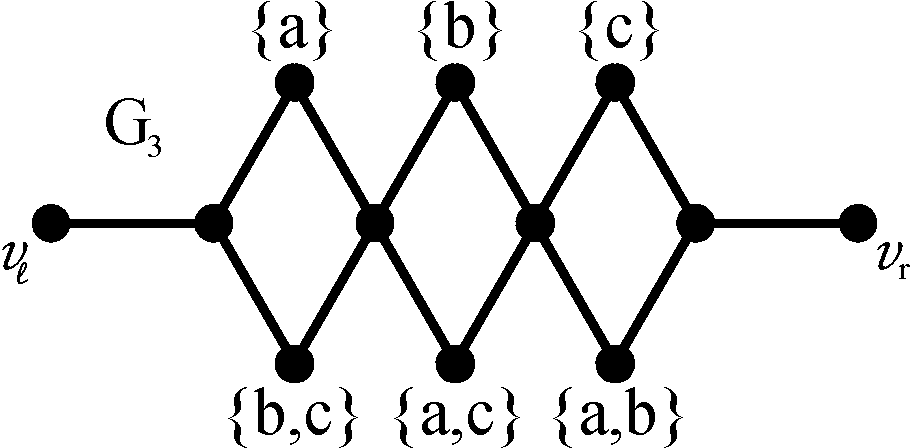
\includegraphics[width=0.3\textwidth,keepaspectratio]{centrsampl/figures/eps/tight-mapexample}
    }
  \hfill
  \subcaptionbox{Graph $G$ with $\VC\left((\mathbb{S}_G,\range_G)\right)=
  3$.\label{fig:centrsampluniquetight}}{
    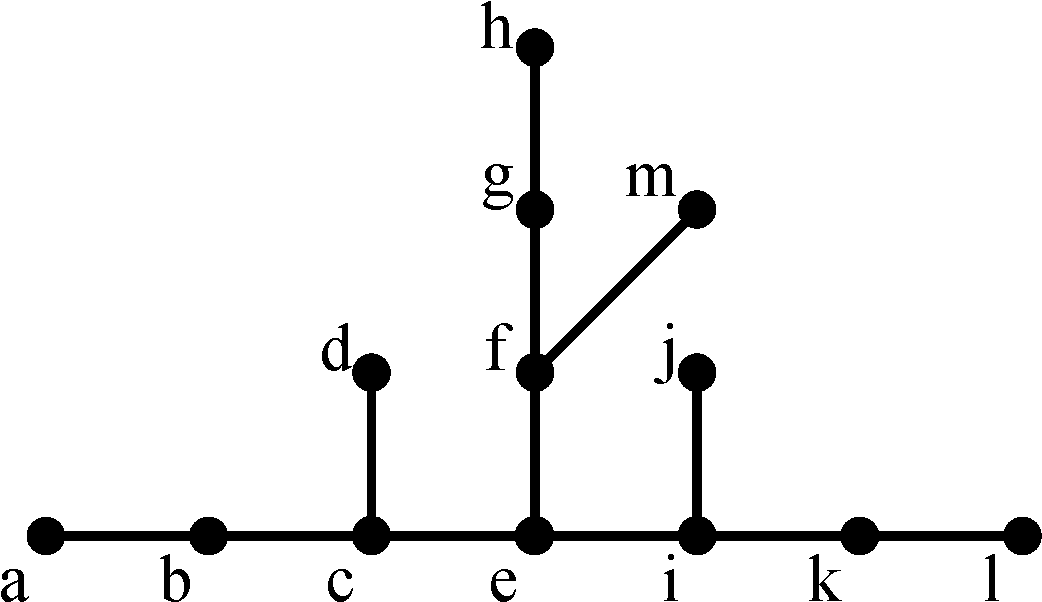
\includegraphics[width=0.3\textwidth,keepaspectratio]{centrsampl/figures/eps/uniqueshortestpathtight}
    }
  \caption{Graphs for which the bound is tight.}
\end{figure}

\begin{lemma}\label{lem:vcdimlowbound}
  $\VC\left((\mathbb{S}_{G_d}R_{G_d})\right)=d$.
\end{lemma}
\begin{proof}
  As we said, the $d$ paths in $Q$  go from $v_\ell$ to $v_\mathrm{r}$.
  From this and the definition of $G_d$ it should be clear that they must go through
  all the middle vertices of $G_d$. Consider now the set
  $S=2^Q\setminus\{Q,\emptyset\}$. We now build a map $\mathsf{r}$
  from the elements of $S$ to the set of top and bottom vertices of $G_d$. We can
  partition $S$ in two sets $A$ and $B$ as follows: %such that $A\cap
  %B=\emptyset$ and $A\cup B=Q$ in the following way: 
  for each unordered pair $(s',s'')$ of
  elements in $S$ such that $s'\cap s''=\emptyset$ and $s'\cup s''=Q$
  we put $s'$ in $A$ and $s''$ in $B$. It is
  easy to see that the size of $A$ ($|A|=2^{d-1}-1$) equals the number of top
  vertices of $G_d$, and analogously for $B$ and the number of bottom vertices.
  The bijection $\mathsf{r}$ will map the
  elements of $A$ to the top vertices of $G_d$ and the elements of $B$ to the
  bottom vertices. For each $s'\in A$, let $\mathsf{c}(s')$ be the unique element $s''$
  of $B$ such that $s'\cap s''=\emptyset$ and $s'\cup s''=Q$ (i.e.,
  $\mathsf{c}(s')=Q\setminus s'$). 
  Let $\mathsf{r}_A$ be an arbitrary one-to-one map from the elements of $A$ to
  the top vertices of $G_d$. Consider now the inverse map $\mathsf{r}^{-1}_A$
  from the top vertices to the elements of $A$. We can create another map
  $\mathsf{r}_B$ from $B$ to the
  bottom vertices of $G_d$ that maps the element
  $\mathsf{c}(\mathsf{r}^{-1}_A(v))$ of $B$ to the bottom vertex $\mathsf{f}(v)$
  corresponding to $v$, for each top vertex $v$. A path $p\in Q$ goes through
  a top vertex $v$ if and only if $p\in\mathsf{r}^{-1}_A(v)$. Analogously, $p$
  goes through a bottom vertex $u$ if and only if $p\in\mathsf{r}^{-1}_B(u)$.
  It is easy to see that, if we combine $\mathsf{r}_A$ and
  $\mathsf{r}_B$, we obtain a map $\mathsf{r}$ from $S$ to the set of
  top and bottom vertices of $G_d$. An example of a possible $\mathsf{r}$ for
  $G_3$ is presented in Fig.~\ref{fig:centrsamplmapexample}.
  We now show that for each $s\in S$, $s=Q\cap\mathcal{T}_{\mathsf{r}(s)}$. This
  is easy to see as $\mathsf{r}(s)$ is internal to all paths in $s$, by
  definition of $\mathsf{r}(s)$ and of the paths in $Q$. On the other end, no
  path from $\mathsf{c}(s)$ goes through $\mathsf{r}(s)$ because it goes through
  the corresponding vertex of $\mathsf{r}(s)$ (top if $\mathsf{r}(s)$ is a
  bottom vertex, bottom otherwise). It is also straightforward to see that,
  if we let $v_Q$ be any arbitrary middle vertex different from $v_\ell$
  or $v_\mathrm{r}$, we have $Q=Q\cap\mathcal{T}_{v_Q}$, given that all paths in
  $Q$ go through all the middle vertices. Also, given that $v_\ell$ is not
  internal to any path, we have $\emptyset=Q\cap\mathcal{T}_{v_\ell}$. Then all
  subsets of $Q$ can be expressed as the intersection between $Q$ and a range
  from $\range_{G_d}$, which means that $Q$ can be shattered and therefore
  $\VC\left((\mathbb{S}_G,\range_{G_d})\right)\ge d$.

  From Lemma~\ref{lem:vcdimuppbound} we know that
  $\VC\left((\mathbb{S}_G,\range_{G_d})\right)\le d$, so
  it must be $\VC\left((\mathbb{S}_G,\range_{G_d})\right)=d$.
\end{proof}

The upper bound presented in Lemma~\ref{lem:vcdimuppboundunique}  for the case
of unique shortest paths is also strict in the same sense.

\begin{lemma}\label{lem:vcdimlowboundunique}
  There is a graph $G=(V,E)$ with $|\mathcal{S}_{uv}|\le1$ for all
  pairs $(u,v)\in V\times V$ such that the range space $(\mathbb{S}_G,\range_G)$ associated to the
  shortest paths in $G$ has VC-Dimension exactly $3$.
\end{lemma}


\begin{proof}
  Consider the graph $G$ in Fig.~\ref{fig:centrsampluniquetight}.
  Let $p_1=(a,b,c,e,i,j)$, $p_2=(m,f,e,i,k,l)$, $p_3=(d,c,e,f,g,h)$ be three
  paths. We now show that $Q=\{p_1,p_2,p_3\}$ can be shattered by $\range_G$, which
  implies $\VC\left((\mathbb{S}_G,\range_G)\right)\ge 3$. We have $\emptyset=Q\cap\mathcal{T}_a$,
  $\{p_1\}=Q\cap\mathcal{T}_b$, $\{p_2\}=Q\cap\mathcal{T}_k$,
  $\{p_3\}=Q\cap\mathcal{T}_g$, $\{p_1,p_2\}=Q\cap\mathcal{T}_i$,
  $\{p_1,p_3\}=Q\cap\mathcal{T}_c$, $\{p_2,p_3\}=Q\cap\mathcal{T}_f$,
  $\{p_1,p_2,p_3\}=Q\cap\mathcal{T}_e$,  
  Hence all subsets of $Q$ can be expressed as the intersection between $Q$ and
  some range in $\range_G$ which means that $Q$ can be shattered and
  $\VC\left((\mathbb{S}_G,\range_G)\right)\ge 3$. Lemma~\ref{lem:vcdimuppboundunique} gives us an upper
  bound $\VC\left((\mathbb{S}_G,\range_G)\right)\le3$, so we can conclude that
  $\VC\left((\mathbb{S}_G,\range_G)\right)=3$.
\end{proof}

Although the example in Fig.~\ref{fig:uniquetight} is a tree, this is not a
requirement for either Lemma~\ref{lem:vcdimuppboundunique} or
Lemma~\ref{lem:vcdimlowboundunique}: in a weighted graph with cycles (i.e., not
a tree) the weights may be such that there is a unique shortest path between any
pair of connected vertices.

